\section{Attribute-Slice Heatmaps}
\label{app:attribute-slice-heatmaps}

Figure~\ref{fig:coco-ratio05-attribute-delta} reports the corresponding
ratio-$0.5$ COCO pose-estimation slice analysis over the full annotated
attribute vocabulary. The targeted repair values are clothes color brown and
rainy weather. As in the ImageNet10 example, the largest gains appear on the
targeted values, while the remaining attributes show smaller changes.

\begin{figure}[p]
\centering
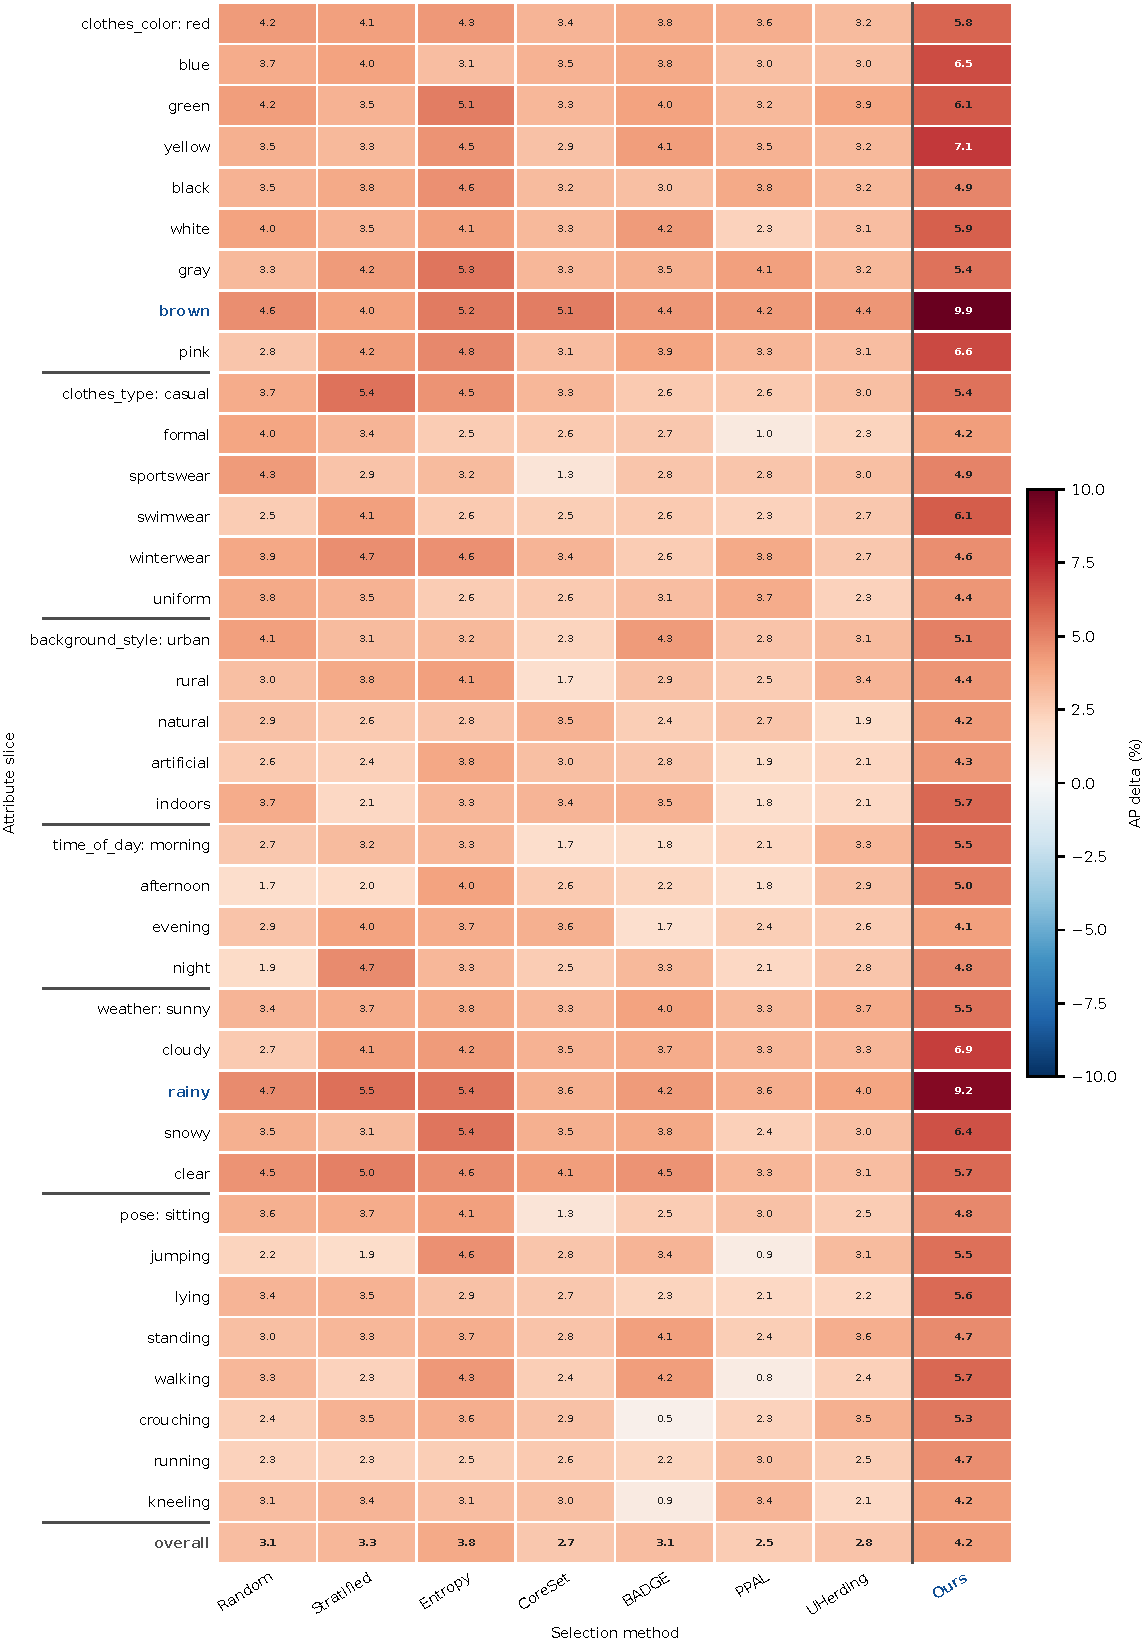
\includegraphics[width=\linewidth]{figures/show/coco_ratio0p5_show_heatmap.pdf}
\caption{COCO pose-estimation ratio-$0.5$ attribute-slice AP deltas. The figure expands the slice-level analysis to all annotated COCO pose-estimation attribute groups. The targeted repair values are clothes color brown and rainy weather.}
\label{fig:coco-ratio05-attribute-delta}
\end{figure}

